%label:"fig:APullbackOfAZeroCycleMayNotBeZero"
%type:"figure"
%name:"a pullback of a zero cycle may not be zero. "
%caption:""
%parent:"art_RationalEquivalenceInTropicalGeometry"


        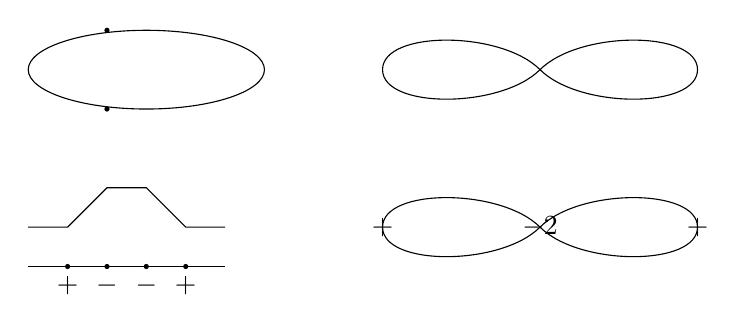
\begin{tikzpicture}


            \draw  (-2.5,0.5) ellipse (1.5 and 0.5);
            \draw (2.5,0.5) .. controls (2,0) and (0.5,0) .. (0.5,0.5) .. controls (0.5,1) and (2,1) .. (2.5,0.5) .. controls (3,0) and (4.5,0) .. (4.5,0.5) .. controls (4.5,1) and (3,1) .. (2.5,0.5);
            \node[circle, scale=.2, fill] at (-3,1) {};
            \node[circle, scale=.2, fill] at (-3,0) {};
            \draw (-4,-2) -- (-1.5,-2);
            \draw (-4,-1.5) -- (-3.5,-1.5) -- (-3,-1) -- (-2.5,-1) -- (-2,-1.5) -- (-1.5,-1.5);
            \node[circle, scale=.2, fill] at (-3.5,-2) {};
            \node[circle, scale=.2, fill] at (-3,-2) {};
            \node[circle, scale=.2, fill] at (-2,-2) {};
            \node[circle, scale=.2, fill] at (-2.5,-2) {};
            
            
            \node[below] at (-3.5,-2) {$+$};
            \node[below] at (-3,-2) {$-$};
            \node[below] at (-2,-2) {$+$};
            \node[below] at (-2.5,-2) {$-$};
            
            \begin{scope}[shift={(0,-2)}]
            \draw (2.5,0.5) .. controls (2,0) and (0.5,0) .. (0.5,0.5) .. controls (0.5,1) and (2,1) .. (2.5,0.5) .. controls (3,0) and (4.5,0) .. (4.5,0.5) .. controls (4.5,1) and (3,1) .. (2.5,0.5);
            
            \end{scope}
            
            \node at (0.5,-1.5) {$+$};
            \node at (4.5,-1.5) {$+$};
            \node at (2.5,-1.5) {$-2$};
            \end{tikzpicture}

